In this chapter, a generic workflow for solving problems of objects detection and classification in images is presented. The history of this workflow is presented in Section \ref{sec:history_first_dev}. Section \ref{sec:workflow_principle} introduces the workflow itself. Finally, the implementation carried out in the context of this thesis is presented and discussed in Section \ref{sec:workflow_impl}.

\section{History and first developments}
\label{sec:history_first_dev}
The Segment-Locate-Dispatch-Classify (SLDC) workflow was first imagined by ?? Jean-Michel Begon ?? as a generalization of the work on thyroid nodule malignancy detection made in \cite{adeblire2013}. In the context of his master thesis, the author had implemented a processing workflow for detecting cells with inclusion and proliferative architectural patterns (see ?? (thyroid)) in digitized thyroid punctions slides. The cells and architectural patterns were detected by segmenting the images and then classified using machine learning techniques. As explained in the Section ?? (thyroid), some patterns could themselves contain cells with inclusion. Therefore, the author implemented a second processing workflow to detect those cells. This workflow was similar to the first because it relied on a segmentation algorithm to isolate cells in patterns and then used machine learning to assess their malignity. 

From those workflows, a common pattern emerged: performing detection using a segmentation algorithm and then classifying the detected objects using machine learning techniques. In 2015, ?? Jean-Michel Begon ?? developed a first version of a generic workflow based on this pattern and gave it the name \textit{Segment-Locate-Dispatch-Classify}. Then, he applied its workflow to the thyroid case. Unfortunately, this implementation suffered from some drawbacks which made it hard to reuse in other contexts. The workflow was therefore re-worked in the context of this master thesis.

\section{Principle}
\label{sec:workflow_principle}

\subsection{Algorithm}
\label{ssec:workflow_algo}
The workflow is a meta-algorithm\footnote{In this context, a meta-algorithm is an algorithm that coordinates the execution of other algorithms.} that detects and classifies objects contained in images. Particularly, given a two-dimensional\footnote{A third dimension can be dedicated to the images channel (i.e. 3 channels for RGB images, 4 channels for RGBA images).} image $\mathcal{I}$ as input, it is expected to output the information about the objects of interest contained in this image. Those information include the shape of the object, its location as well as a classification label. Formally, the workflow can be seen as an operator $\mathcal{W}$:

\begin{definition} Let $\mathcal{W}$ be an operator such that 
	\begin{equation}\label{eqn:workflow_operator}
		\mathcal{W}(\cdot) : \mathcal{I} \rightarrow \left\{(o_1,C_1),...,(o_N, C_N)\right\}
	\end{equation}
	where $N$ is the number of objects of interest in $\mathcal{I}$ and $(o_i, C_i)$ is a tuple. The first element of this tuple, $o_i$, is a representation of the information (shape and location) about the $i^{th}$ object of interest found in $\mathcal{I}$ and the second, $C_i$, its classification label. 
\end{definition}

It is worth noting that genericity is of the essence. That is, the meta-algorithm should be able to solve the widest possible range of object detection and classification problems. Moreover, as explained in Section \ref{sec:history_first_dev}, it should produce those outputs using image segmentation and machine learning. As far as the segmentation is concerned, genericity is usually hard to obtain because of the high variability of images across different problems. In order to ensure genericity, the workflow doesn't impose a particular segmentation procedure but expects the implementer to provide one that suits the problem. The same goes for the classification models used for predicting the labels of the objects. 

In the subsequent sections, some additional operators are defined and used to build the $\mathcal{W}$ operator. First, a basic version of the algorithm is presented and then refined in order to achieve an acceptable level of genericity.

\subsection{Additional operators}
\label{ssec:other_operators}

Segmentation is the first operation applied to the image. This step of the algorithm is where the detection is actually carried out:
 
\begin{definition} \label{def:segmentation_op}
Let $\mathcal{S}$ be the \textbf{segment} operator. It is applied to an image $\mathcal{I}$ and produces a binary mask $\mathcal{B}$. The pixel $b_{ij}$ of $\mathcal{B}$ is 1 if the pixel $p_{ij}$ of $\mathcal{I}$ is located in an object of interest, otherwise it is 0. Formally:
\begin{equation}
	\label{eqn:operator_segment}
	\mathcal{S}(\cdot) : \mathcal{I} \rightarrow \mathcal{B}
\end{equation}
\end{definition}

While the segmented image theoretically contains the necessary information about the detected objects (i.e. shape and position in the image), the format of this information is inconvenient to query mostly because it is embedded into the binary mask and a single object cannot be trivially extracted. An intermediate step that would convert this information into a more convenient format is therefore needed. This format should encode both the shape of the object and its position in the image. It appears that polygons match this specification. 

\begin{definition} \label{def:locate_op}
Let $\mathcal{L}$ be the \textbf{location} operator. It is applied to a binary mask and produces a set of polygons encoding the shapes and positions of every object in the image. Formally:

\begin{equation}
	\mathcal{L}(\cdot) : \mathcal{B} \rightarrow \left\{P_1, ..., P_N\right\}
\end{equation}

where $\mathcal{B}$ is a binary mask as defined in Definition \ref{def:segmentation_op}, $N$ is the number of objects of interest in $\mathcal{B}$ and $P_i$ is the polygon representing the geometrical contour of the $i^{th}$ object in $\mathcal{B}$.
\end{definition}

The final step of the workflow is the object classification and is performed by a classifier which is passed a representation of the object (e.g. image, geometrical information,...) and produces a classification label. In this theory, there is no restriction about the nature or representation of the objects processed by the classifiers.

\begin{definition} \label{def:classif_op}
Let $\mathcal{T}$ be the \textbf{classifier} operator. It is applied to an object of interest and produces a classification label. Formally:
\begin{equation}
	\mathcal{T}(\cdot) : o \rightarrow C
\end{equation}
where $o$ is the object and $C$, the classification label. 
\end{definition}
\begin{definition}
Let $\mathcal{T}^*$ be an extension of $\mathcal{T}$ which is given a set of objects and produces labels for all of them. Formally: 
\begin{equation}
	\mathcal{T}^*(\cdot) : \left\{o_1, ..., o_N\right\}  \rightarrow \left\{C_1, ..., C_N\right\}
\end{equation}
\end{definition}

\subsection{Single segmentation, single classifier}
\label{ssec:single_single}

The most simple construction of $\mathcal{W}$ would be the composition of the operators defined in Section \ref{ssec:other_operators}. Particularly, the compositions $\mathcal{S} \circ \mathcal{L}$ and $\mathcal{S} \circ \mathcal{L} \circ \mathcal{T}^*$ would respectively produce the polygons representing the objects and and their labels. This construction is summarized in Algorithm \ref{algo:single_seg_single_classif}: 

\begin{algorithm} \label{algo:single_seg_single_classif} 
	Construction of $\mathcal{W}$ using one segmentation and one classifier:
	
	\begin{enumerate}
		\item Return $\left(\mathcal{S} \circ \mathcal{L}\right)\left(\mathcal{I}\right) \times \left(\mathcal{S} \circ \mathcal{L} \circ \mathcal{T}^*\right)\left(\mathcal{I}\right)$
	\end{enumerate}
\end{algorithm}

As explained in Section \ref{ssec:workflow_algo}, the definition of $\mathcal{S}$ and $\mathcal{T}^*$ would be left at the implementer's hands. As far as the $\mathcal{L}$ operator is concerned, it could be imposed by the workflow without loss of genericity. Such a construction of $\mathcal{W}$ could already solve any object detection and classification problem on image in which the labels can be predicted by a single classifier. However, in some cases, one classifier is not enough. This happen, for instance, when the image contains objects of very different nature and using several classifiers would yield better results than using a single one. An extension is therefore needed.

\subsection{Single segmentation, several classifiers}
\label{ssec:single_several}

In this attempt to construct a generic $\mathcal{W}$ operator, the image is assumed to contain $M$ distinct types of objects and the workflow uses $M$ classifiers (the $i^{th}$ classifier being noted $\mathcal{T}_i$ with $i \in \{1,...,M\}$) to classify those objects. As an object should only be processed by one classifier, the workflow has to be added a new step which consists in dispatching each polygon to its most appropriate classifier. 

\begin{definition}\label{def:dispatch_op} 
	Let $\mathcal{D}$ be the dispatch operator. It is applied to a polygon and produces an integer which identifies the most appropriate classifier for processing this polygon: 

	\begin{equation}
		\mathcal{D}(\cdot) : P \rightarrow i, i \in \{1,...,M\}
	\end{equation}
\end{definition}

This step being problem dependent, it is the responsibility of the implementer to define the rules used for dispatching the polygons. However, the format of these rules can be defined.

\begin{definition} 
	Let $\mathcal{P}$ be a set of $M$ predicates $p_1, ..., p_M$ which associate truth values to polygons:
	\begin{equation}
		p_i(\cdot) : P \rightarrow t \in \{true, false\}, i \in \left\{1,...,M\right\} 
	\end{equation}
	where $p_i$ is the predicate associated with the $i^{th}$ classifier. The polygon $P$ is dispatched to a classifier $\mathcal{T}_i$ if $p_i$ associates true to this polygon. To avoid dispatching an object to several classifier, the predicates should verify the following property:
	\begin{equation}
		p_i = true \Leftrightarrow p_j = false, \forall j \neq i
	\end{equation} 
\end{definition}

Given this format, the $\mathcal{D}$ operator can be trivially constructed as it returns $i$ if $p_i$ is \textit{true}. The algorithm resulting from this construction of $\mathcal{W}$ starts the same way as in Section \ref{ssec:single_single}: the image is applied the segment and locate operators. Then, the resulting polygons are dispatched and classified to produce the classification label. The resulting algorithm is summarized in Algorithm \ref{algo:single_seg_several_classif}. 

While the range of problems that can be solved using this algorithm has been increased compared to the version with a single classifier, there are still some problems that cannot be. In particular, if some objects are included into other bigger objects, they won't be considered as independent objects. 

Before extending the algorithm for handling this case, it is worth noting that Algorithm \ref{algo:single_seg_several_classif} is completely compatible with Algorithm \ref{algo:single_seg_single_classif}. Indeed, if there is only one classifier (i.e. $M = 1$) and the predicate $p_1$ always returns $true$, then both algorithms are exactly the same. 

\begin{algorithm}\label{algo:single_seg_several_classif}
Construction of the $\mathcal{W}$ operator with a single segmentation and several classifiers. 
\begin{enumerate}
	\item Apply the $\mathcal{S} \circ \mathcal{L}$ composition to the input image $\mathcal{I}$ to extract the objects of interest as the set of polygons $S_p \leftarrow \left\{P_1, ..., P_N \right\}$
	\item Initialize the labels set $L \leftarrow \emptyset$
	\item For each polygon $P \in S_p$:
	\begin{enumerate}
		\item Compute the classification label $C \leftarrow \mathcal{T}_{\mathcal{D}(P)}(P)$
		\item Place the label in the labels set $L \leftarrow L \cup \{C\}$
	\end{enumerate}
	\item Build and return objects and labels set $S_p \times L$.
\end{enumerate}
\end{algorithm}

\subsection{Chaining workflows}

To handle the case when objects of interest can be included into objects of bigger size in the image, a solution consists in executing several instances of Algorithm \ref{algo:single_seg_several_classif} one after another. 

\begin{definition}\label{def:several_w_op}
	Let $\mathcal{W}_1, ..., \mathcal{W}_K$ be a set of $K$ instances of Algorithm \ref{algo:single_seg_several_classif}. Each algorithm $\mathcal{W}_i$ has its own segmentation procedure $\mathcal{S}_i$ and proper sets of dispatching predicates $\mathcal{P}_i$ and classifiers $S_{\mathcal{T},i}$.
\end{definition}

While $\mathcal{W}_1$ would be applied to the full image $\mathcal{I}$ to extract all the objects of interest, $\mathcal{W}_2, ..., \mathcal{W}_K$ would only be passed image windows containing the previously detected objects and would have to detect the objects of intereset included in the objects found by $\mathcal{W}_1$. 

\begin{definition}\label{def:image_window}
	Let $\mathcal{I}_P$ be an image window extracted from image $\mathcal{I}$ and containing the object represented by polygon $P$. The window is the minimum bounding box containing this polygon.
\end{definition}

A further refinement would be to provide a way for the implementer to filter the polygons of which the windows are passed to a given workflow instance. Indeed, a given instance $\mathcal{W}_i$ might be designed to process only a certain category of objects and therefore should not be passed windows of objects that doesn't fall in this category. 

\begin{definition}\label{def:filter_op}
	Let $\mathcal{F}$ be the $\textbf{filter}$ operator. It is given a set of polygons $S_P$ and returns a subset $S'_P$ of polygons:
	
	\begin{equation}
		\mathcal{F}(\cdot): S_P \rightarrow S'_P, S'_P \subseteq S_P
	\end{equation}
\end{definition}

Each instance of the workflow $\mathcal{W}_i$ except $\mathcal{W}_1$ is therefore associated a filter operator $\mathcal{F}_i$. The resulting algorithm is given in Algorithm \ref{algo:chaining_workflows} and has now reached an acceptable level of genericity.

\begin{algorithm} \label{algo:chaining_workflows}
	Construction of the $\mathcal{W}$ operator with $K$ instances of Algorithm \ref{algo:single_seg_several_classif}:

	\begin{enumerate}
		\item Execute the first workflow and save the results in the results set $R$: $R \leftarrow \mathcal{W}_1(\mathcal{I})$
		\item Create the polygons set and initializes it with the polygons found from the execution of $\mathcal{W}_1$: $S_P \leftarrow \left\{P_1, ..., P_N\right\}$
		\item For each $i \in \{2, ..., K\}$:
		\begin{enumerate}
			\item Extract polygons to be processed by $\mathcal{W}_i$: $S'_P \leftarrow \mathcal{F}_i(S_P)$
			\item For polygon $P \in S'_P$:
			\begin{enumerate}
				\item Execute workflow $\mathcal{W}_i$ on the image window and saves the results: $R \leftarrow R \cup \mathcal{W}_i(\mathcal{I}_P)$
				\item Add the extracted polygons to the polygons set: $S_P \leftarrow S_P \cup \left\{P_1, ..., P_M\right\}$
			\end{enumerate}
		\end{enumerate}
		\item Return the results set $R$
	\end{enumerate}
\end{algorithm}

\section{Implementation}
\label{sec:workflow_impl}
This section aims at presenting the implementation of the workflow developed in Section \ref{sec:workflow_principle}. In Section \ref{ssec:work_init_impl}, the reasons why the previous implementation was replaced by a new one are presented. Then, the requirements, design choices and architecture of the new framework\footnote{In this section, the term \textit{workflow} will refer to the algorithm while \textit{framework} will refer to the implementation.} are given in Sections \ref{ssec:work_requirements}, \ref{ssec:work_language} and \ref{ssec:work_arch}. Finally, how to apply the framework is illustrated with a toy example in Section \ref{ssec:work_toy_example}. The framework discussed in this section is available on GitHub ?? at \href{https://github.com/waliens/sldc}{this url} ??.

\subsection{Initial implementation}
\label{ssec:work_init_impl}
As explained in \ref{sec:history_first_dev}, a first implementation of the workflow was done in 2015. However, in the context of this thesis, the decision was made to re-implement it for various reasons.

A major issue was the presence of a software component called a \textit{datastore} which had to be implemented for each application of the workflow. In addition to be a dependency of almost every other class of the framework, it actually forced the implementer to define workflow execution and chaining logic himself although this logic is obviously not problem dependent and could be encapsulated. The major consequence of this design was an increased workload for the implementer to apply the framework to a custom objects detection and classification problem. Moreover, the datastore being tightly coupled with other classes, it made it almost impossible to unit test the framework and to reproduce bugs.

Another issue with the previous implementation was its too high level of genericity. Most of the components of the framework were defined as abstract classes and interfaces to be derived or implemented to apply the workflow to a custom problem. This made the framework hardly understandable and difficult to apply as the implementer would have to define more than just problem dependent components. In some cases, some implementations were provided but they only increased the complexity of the framework. Indeed, it was not clear whether those classes could be used directly or whether the implementer should provide his own classes.

Another final critical point was the lack of robustness. Especially, when applied to the thyroid case where images were fetched using HTTP requests, any network error would exit the program, leading to the loss of all collected data.

All in all, it was decided to re-implement the framework to get rid of those issues. However, it was not decided to restart from scratch as the good parts of the existing work were kept. The philosophy behind the new framework is illustrated through a set of requirements in Section \ref{ssec:work_requirements}.

\subsection{Requirements}
\label{ssec:work_requirements}
The main requirements for the framework are listed hereafter.

\paragraph{Genericity} As for the algorithm, the framework should be able to solve the widest possible range of objects detection and classification problems in any context. This property has more implication in the case of the framework design than for the algorithm design, especially when it comes to fixing the representation of the various involved data types (i.e. image, polygon,...).

\paragraph{Efficiency} While the framework has no control over the efficiency of the algorithms defined by the implementer (i.e. segmentation or classification procedures), the coordination of those algorithms should not induce a significant overhead in the overall execution. 

\paragraph{Large images} While large images handling was irrelevant at the algorithm design stage, it becomes critical at this point. To remain generic, the framework should not make any assumption about the size of the images to be processed. Especially, a whole image should not be assumed to fit into memory.

\paragraph{Robustness} The framework should be robust to errors. That is, a single error should not interrupt the whole execution. For instance, if the framework executes a set of independent computations and one of them fails, it should only be stopped if this failure is unrecoverable and affects all the other computations. Otherwise, the failure should be reported and those others computations should execute until completion. 

\paragraph{Transparency} The framework should provide a built-in way to communicate its progress, the duration of each steps as well as the errors it encounters with the user. The level of verbosity of this communication tool should be adjustable. 

\paragraph{Parallelism} Whenever possible the framework should take advantage of parallelism to reduce its execution time but the implementer should be given a way to switch to sequential execution. Moreover, the implementer should be able to adjust the level of parallelism (i.e. the number of available processors).

\paragraph{Ease of use} The work of the implementer should be kept as minimal as possible. He should only have to define the logic of the workflow components that are problem dependent : segmentation, dispatching rules, classifiers,... 

\subsection{Language}
\label{ssec:work_language}
The first design choice occurring in the implementation of an existing algorithm is obviously the language in which this implementation will be made. As far as the workflow is concerned, the chosen language was Python. Indeed, this language provides a very complete environment for developing objects detection and segmentation algorithms which would obviously contribute to the overall ease of use the framework. 

First of all, the language has many features which allows developers to quickly come up with solutions to problems. Especially, it is strongly and dynamically typed, multi-paradigm (imperative, functional, object oriented,...), interactive (it can be used in an interactive console), interpreted and garbage-collected. It also support usual data structures such as lists, arrays, dictionaries and sets natively and provide operations for manipulating them in a concise way. 

In addition to its built-in features, Python has become a great language for scientific computing as it has been augmented with excellent open source libraries over the years. First, the SciPy ecosystem which includes the SciPy \cite{oliphant:2007} and NumPy \cite{vanderwalt:2011} libraries. The first is a collection of numerical algorithms and domain-specific toolboxes (signal processing, optimization, statistics,...). The second is a fundamental package for numerical computations which provides an efficient representation of multi-dimensional arrays and operations on them. Built on top of the SciPy ecosystem comes Scikit-Learn \cite{pedregosa:2011}, a library that provides simple, efficient and reusable tools for data mining and machine learning. Image processing is not outdone with a Python binding for the huge OpenCV library \cite{opencv_library}. Two alternatives are scikit-image \cite{scikit-image} which is built on top of the SciPy ecosystem or the Pillow library \cite{pillow}. All of them provide a collection of well-known image processing algorithms. Another useful library is Shapely \cite{shapely} which provides a representation for geometrical objects such as polygons as well as operations to apply on them. 

Python was also chosen because the workflow was implemented to be integrated with Cytomine (see Section ??). Particularly, the final goal was the detection and classification of objects in images stored on Cytomine servers. As those images and their metadata are exposed through an API interfaced by a Python client, it was essential that the workflow could use this client to communicate with the back-end. As the Cytomine client was implemented in the version 2.7.11 of Python, this version was also used for developing the framework. 

\subsection{Software architecture}
\label{ssec:work_arch}
As one of the main goal of this implementation is to reuse it for solving other problems, the framework was implemented as a Python library and released on GitHub ?? url ??.

To ensure code modularity, classes were organized in packages. To prevent any name clashes with other Python libraries, those packages were placed in a root package called \texttt{sldc}. 

\subsubsection{Image representation} 
\label{sssec:work_image_repr}
The image representation design is a critical point of the framework architecture. Indeed, on the one hand, it should be abstract enough so that implementers can apply the workflow on images in any format. On the other hand, it should provide access to a concrete representation available to the framework. Indeed, some steps need to access this representation to extract some information. For instance, location is one such step as it processes a binary mask to extract polygons. 

The representation should also provide a way of extracting sub-windows from an image. The need for this feature is twofold. First, it is needed by the workflow (see Definition \ref{def:image_window}). Then, it could be used to address the large images handling requirement and to overcome the fact that a whole image is not assumed to fit into memory. The idea is to split an image into smaller chunks called tiles which could be loaded into memory and processed one after another. Especially, the tiles would be applied the first part of the workflow that is segmentation and location. As the polygons of each tile are extracted independently, it might occur that a single object of interest which spreads over several tiles ends up being splitted into several polygons. To make sure there is a one to one relationship between a polygon and an object of interest, an additional step must be added to the workflow before the dispatching and would consist in merging the polygons representing a same object. This step is detailed in Section \ref{sssec:merging}.

The abstract image representation and related classes were implemented into the \texttt{sldc.image} package presented in the UML diagram shown in Figure \ref{fig:uml_image_package}.

The \texttt{Image} class is the abstract image representation mentioned above. It provides three abstract methods for checking image dimensions (width, height and number of channels) and a fourth one, \texttt{np\_image}, which should implement the conversion between the implementor's custom image format and the concrete format mentioned above. NumPy multi-dimensional arrays were chosen to be this concrete representation. In addition to the inherent advantage of using the NumPy library, this choice was also motivated by the fact that those arrays are compatible with the various image processing libraries presented in Section \ref{ssec:work_language}. 

An image window is materialized by the \texttt{ImageWindow} class of which the design is based on the decorator pattern. It stores information about the position and size of the window as well as a reference to the parent image. Especially, location and size are respectively represented by coordinates of the first top left pixel included in the window (coordinates are referenced to the top left corner of the parent image) and by the window width and height. As an image window instance provides a level of indirection on top of another image, some methods are provided to fetch the base image as well as the absolute offset\footnote{The absolute offset is the offset of the window referenced to the base image's top left pixel. It is different from the image window offset if its parent image is also an image window.}.

A tile is also represented by a class named \texttt{Tile} which extends \texttt{ImageWindow} and augment it with an integer identifier field. As tiles can potentially be derived, a \texttt{TileBuilder} interface was developed. As suggested by the name, a class implementing this interface is responsible for building specific tile objects. This structure is actually an application of the factory method pattern which has the advantage of allowing the framework to build tile objects defined by the implementer while remaining unaware about the class that will actually be instantiated as well as how it will be instantiated.

Finally, to make it easier to iterate over the tiles of an image two classes were developed : \texttt{TileTopology} and \texttt{TileTopologyIterator}. The first is responsible for dividing an image into a set of overlapping tiles. The overlap allows the merging procedure to be simpler as polygons corresponding to a same object will have a geometrical intersection. 

The tile topology is fully defined with three parameters: the tile maximum width, $w_m$, and height, $h_m$, and the number of pixels that overlap, $o_p$. The tile topology object also associates unique increasing identifiers to the tiles. An example topology with its resulting tiles and identifiers is shown in Figure \ref{fig:tile_topo_example}. As soon as the \texttt{TileTopology} object is built, it can be queried using those identifiers for building tile objects or for fetching topology information such as one tile's neighbours identifiers. While this organization goes off from the object oriented philosophy a bit, it allows all operations provided by the tile topology object to be $\mathcal{O}(1)$ (see Appendix \ref{apdx:tile_topology}). It goes without saying that the overlap parameter should be set carefully because it induces some additional computations. Indeed, some parts of the image will be segmented several times as they are present on more than one tile. 

The second class, \texttt{TileTopologyIterator}, is an application of the iterator design pattern as its name suggests. It can be created either from a tile topology or directly from a subclass of \texttt{Image}. It allows to iterate over the tiles defined by a tile topology. The implementation of this iterator is straightforward. It simply iterates over the tile identifiers and pass them to the corresponding tile topology to build the tiles. 

\begin{figure}[h]
	\center 
	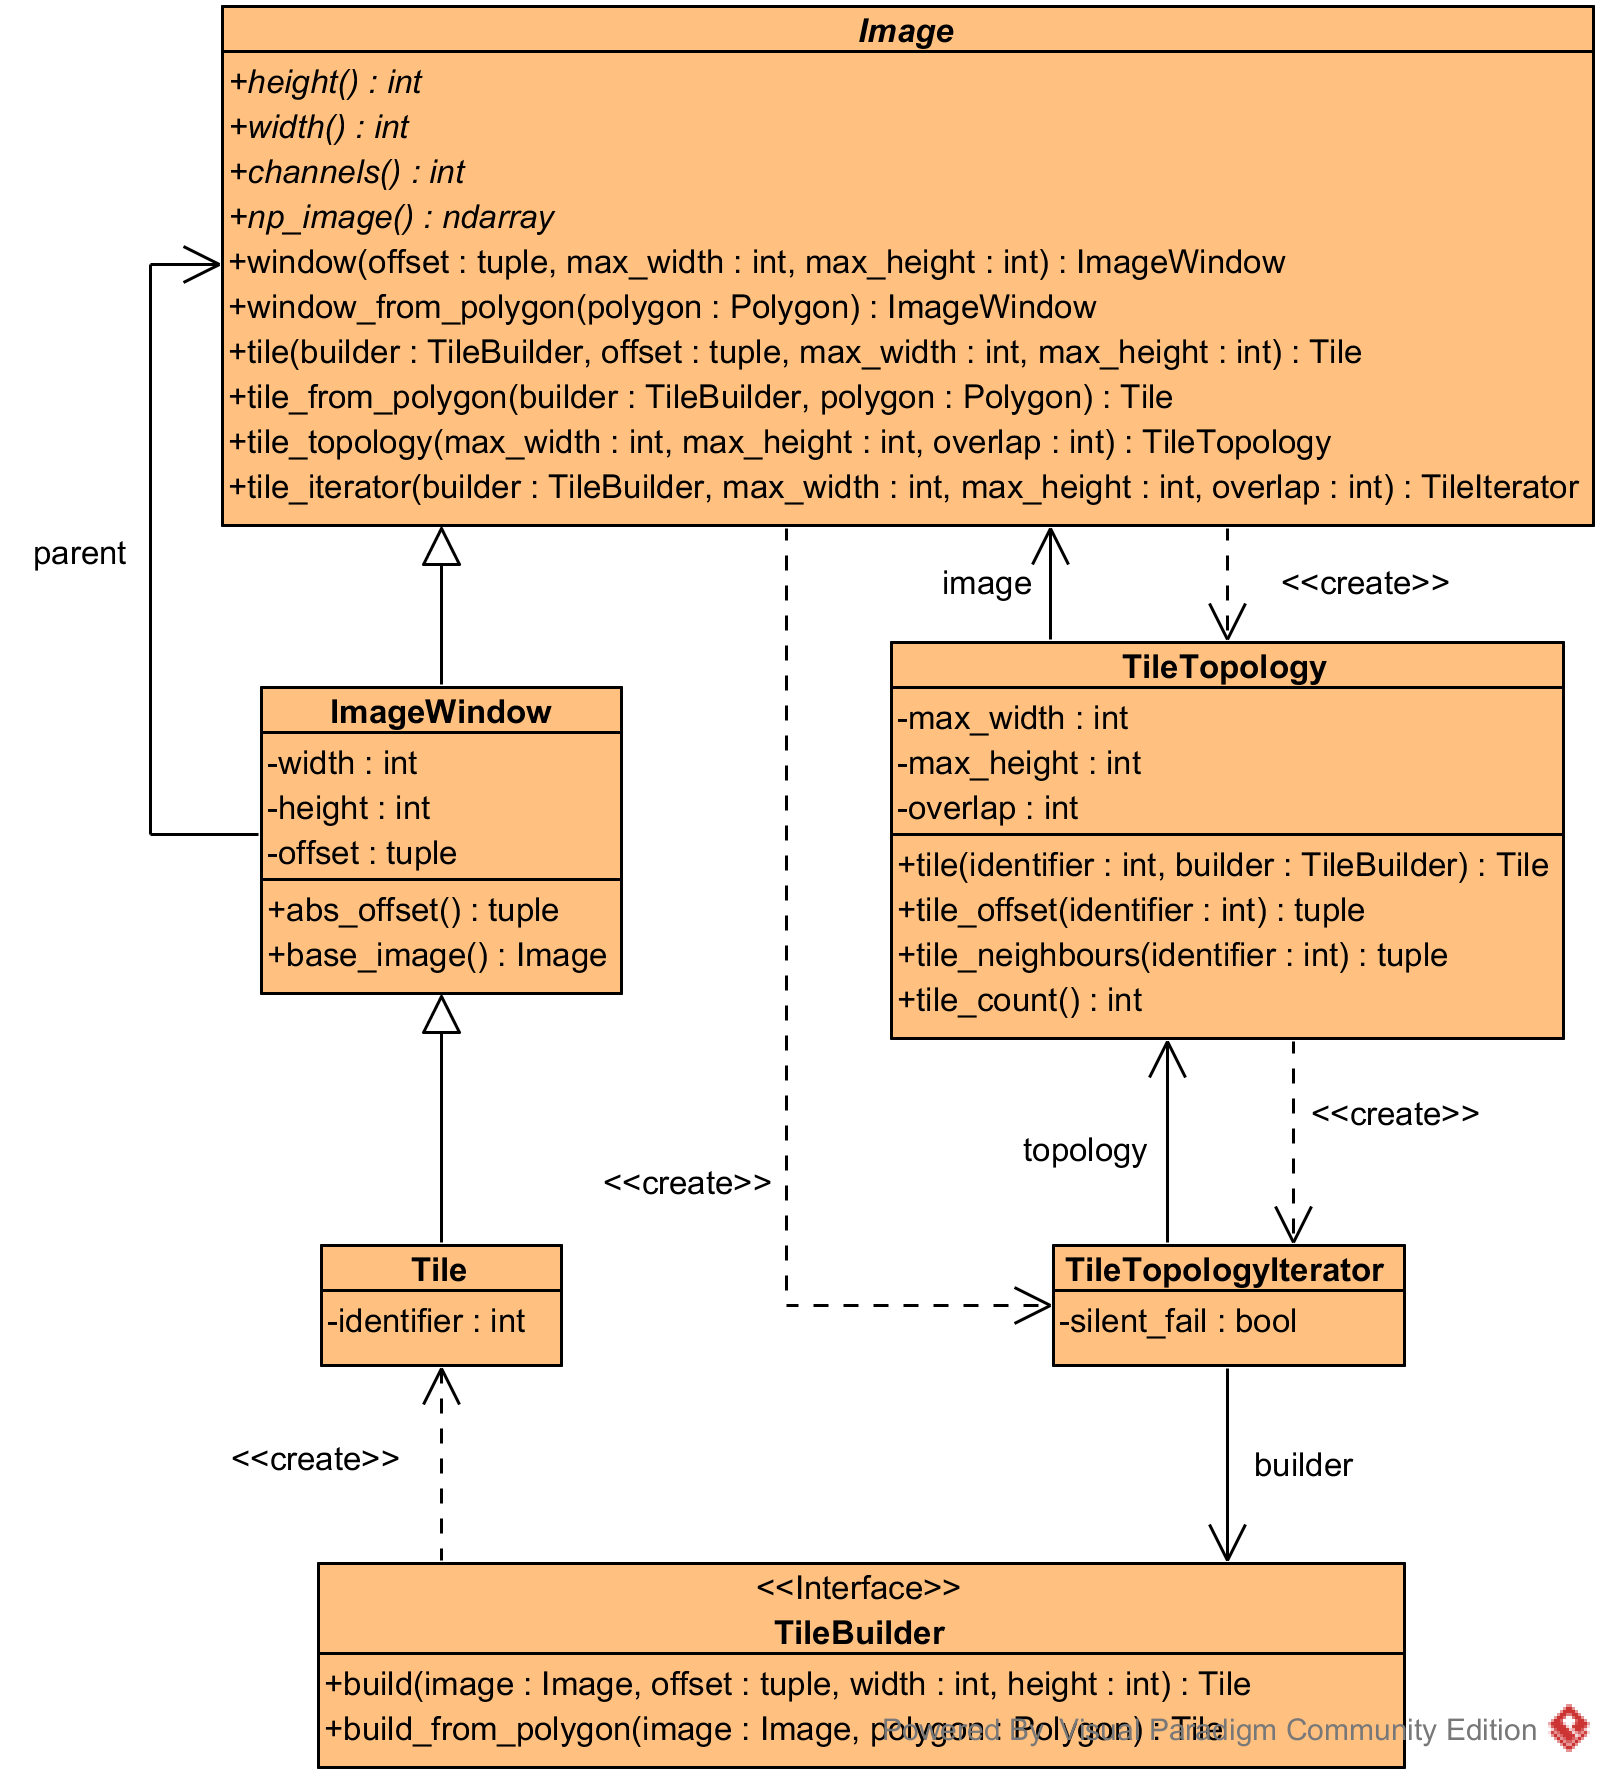
\includegraphics[scale=0.9]{image/uml_image_package.png}
	\caption{Image representation classes - package \texttt{sldc.image}}
	\label{fig:uml_image_package}
\end{figure}

\begin{figure}[h]
	\center
	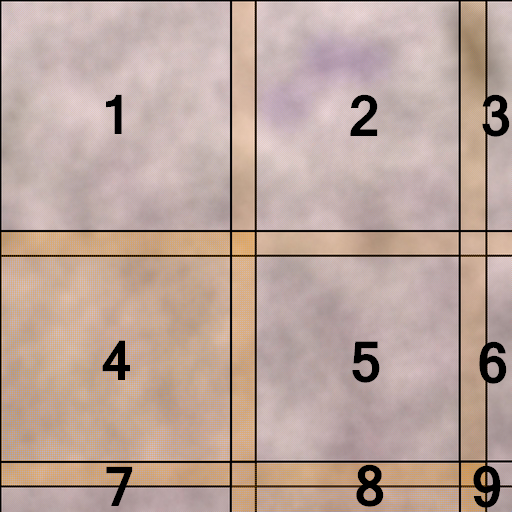
\includegraphics[scale=0.7]{image/tile_topo_2048_2048.png}
	\caption{A tile topology applied on a $512\times 512$ image (parameters: $w_m = 256$, $h_m = 256$ and $o_p = 25$). The numbers are the tile identifiers.}
	\label{fig:tile_topo_example}
\end{figure}

\subsubsection{Segmentation}
As explained in Section \ref{ssec:single_single}, the segmentation is not fixed by the framework and the implementer is expected to provide its own implementation. To represent this constraint in the framework, a \texttt{Segmenter} interface was defined in package \texttt{sldc.segmenter}. It provides a single method, \texttt{segment}, which receives a NumPy representation of the image and is expected to return another NumPy array storing the binary mask marking the objects of interest contained in this image. The binary mask however doesn't conform strictly to Definition \ref{def:segmentation_op} as pixels belonging to an object of interest are marked with the integer value 255 (which corresponds to white in the grayscale color space) instead of 1. The \texttt{Segmenter} interface is Shown in Figure \ref{fig:uml_pack_seg_merg_loc_classif}.

\begin{figure}
	\center 
	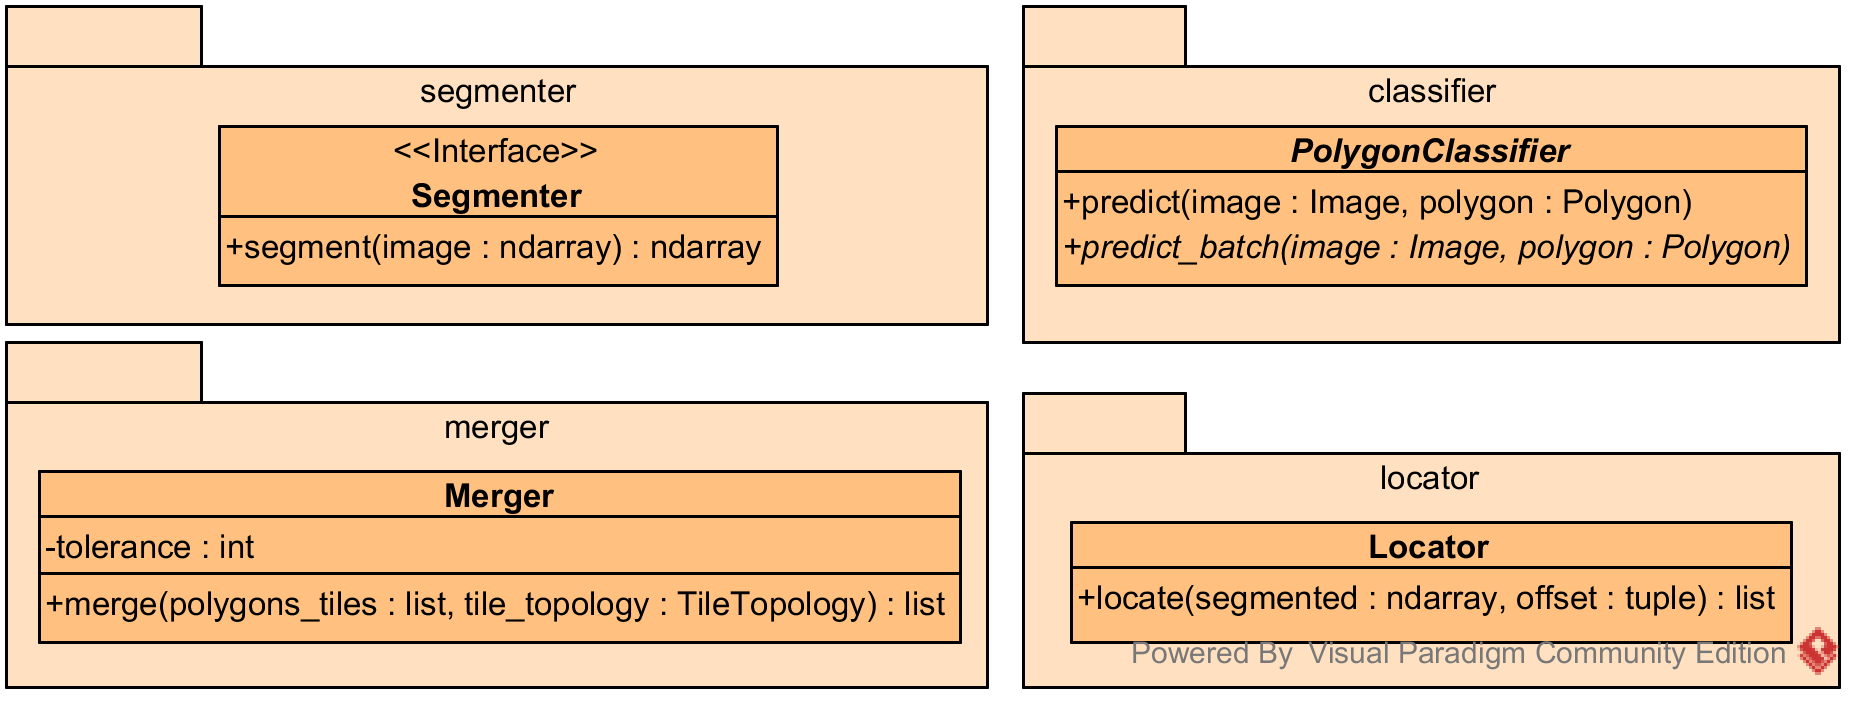
\includegraphics[scale=0.75]{image/uml_seg_merg_loc_classif.png}
	\caption{Packages \texttt{sldc.segmenter}, \texttt{sldc.locator}, \texttt{sldc.merger} and \texttt{sldc.classifier}.}
	\label{fig:uml_pack_seg_merg_loc_classif}
\end{figure}

\subsubsection{Location}
As presented in Definition \ref{def:locate_op}, the location procedure extracts polygons representing the geometrical contours of the objects of interest from a binary mask. The implementation of this operation was done in the single method, \texttt{locate}, of a class called \texttt{Locator} (in package \texttt{sldc.locator}). This method takes as parameter the binary mask represented by a NumPy array and returns the expected set of polygons as Shapely \texttt{Polygon} objects.
 
As stated in Section \ref{ssec:single_single}, this operation can be fixed by the framework without loss of genericity. This is made possible by the choice of representation for the method's inputs and outputs. As far as the implementation is concerned, it was largely inspired from another implementation taken from the Cytomine codebase. It uses the \texttt{findContours} procedure of the OpenCV library to extract the geometrical information of the objects as a list of coordinates. The implementation provided with the framework has two small additions compared to the Cytomine one. The first is the conversion of those coordinates into \texttt{Polygon} objects and the second is an optional translation that can be applied to those polygons. This second modification is needed because of the image division in tiles. Indeed, by default, the location algorithm constructs polygons referenced to the top-left pixel of the binary mask passed to \texttt{locate}. Yet, the polygons are expected to be referenced to the full image top-left pixel. An additional parameter was therefore added to the \texttt{locate} method prototype allowing the caller to specify a translation offset to apply to the found polygons. The \texttt{Locator} class is Shown in Figure \ref{fig:uml_pack_seg_merg_loc_classif}.

\subsubsection{Merging}
\label{sssec:merging}
The need for a merging phase is a consequence of the image division in tiles and its goal is to merge distinct polygons that actually represent a same object of interest. The main idea behind the algorithm was imagined by Jean-Michel Begon. It consists in building a graph where each node corresponds to a polygon. The algorithm will then add edges between polygons which correspond to a same object. Two polygons represent a same object if the distance between them (i.e. minimum distance between one point of each polygon) is less then a certain tolerance threshold. Generating the final polygons is as simple as finding all the connected components of this graph and computing the intersection of all the polygons in those components. 

While working in some cases, the implementation made by Jean-Michel Begon presented some issues. First, the interface of the class was inconvenient to use. Indeed, the tiles and their polygons had to be provided in a fixed order (i.e. increasing order of identifiers). And if they weren't, the merging would fail. Moreover, it had issues with some edge cases. For instance, with small images containing few tiles. For those reasons, the algorithm was kept but was completely reimplemented to take advantage of the \texttt{TileTopology} object (which didn't exist in the previous implementation of the workflow). 

The classes related to merging were defined in the package \texttt{sldc.merger}. The main logic of the algorithm was implemented in a class called \texttt{Merger}. Applying a merge is as simple as passing a tile topology as well a the tiles and associated polygons to the \texttt{merge} method which return the list of merged polygons. The \texttt{Merger} class is Shown in Figure \ref{fig:uml_pack_seg_merg_loc_classif}.

\subsubsection{Dispatching and classification}
As defined in Section \ref{ssec:single_several}, the dispatching of polygons to classifiers is performed using predicates. Those predicates are materialized by the abstract class \texttt{DispatchingRule} in package \texttt{sldc.dispatcher} that the implementer can extend to define custom dispatching logic. Especially, this is done by implementing the method \texttt{evaluate\_batch} which is passed both a list of polygons to dispatch as well as the image from which they were extracted. Passing both the polygons and the image allows the implementer to define a dispatching logic either based on the polygons geometrical properties, or on the image of the object represented by the polygon, or both.  

The same philosophy was followed for classification. The user has to extend the abstract class \texttt{PolygonClassifier} from package \texttt{sldc.classifier} (see Figure \ref{fig:uml_pack_seg_merg_loc_classif}). For the same reason as for the \texttt{evaluate\_batch} method, the \texttt{predict\_batch} methods takes as parameters a set of polygons and the image the they were extracted from. While only a classification labelled is produced by the classifier operator in Definition \ref{def:classif_op}, an additional element is return by the \texttt{predict\_batch} method: the class probability (i.e. the probability that the predicted label is really the label associated with the classified object). Indeed, this information can sometimes be extracted using some specific classifiers. If this information cannot be generated, the implementer can simply return one as probability for each polygon. The class \texttt{PolygonClassifier} is shown in Figure \ref{fig:uml_pack_seg_merg_loc_classif}.

\subsubsection{Workflow}

\subsubsection{Workflow chain}

\subsection{How to use the framework}
\label{ssec:work_toy_example}
A toy example: finding disks in an image with grey background and guessing whether they're black or white 